% !TEX root = C:\Users\Ignacio\Documents\Escuela\CC3002 - Metodologías de Diseño y Programación\apunte-y-ejercicios\src\latex\Apunte.tex
\subsection{Creación de un proyecto}
  Entenderemos por \textbf{proyecto} a cualquier conjunto de archivos y clases que 
  componen una aplicación.
  
  Si es la primera vez que se abre \textit{IntelliJ}, entonces se mostrará el 
  \textit{landing view} del \textit{IDE}, ahí pueden crear un nuevo proyecto 
  directamente haciendo clic en la opción \texttt{Create New Project} (vean la figura 
  \ref{fig:intellij-lv}).

  \begin{figure}[ht!]
    \centering
    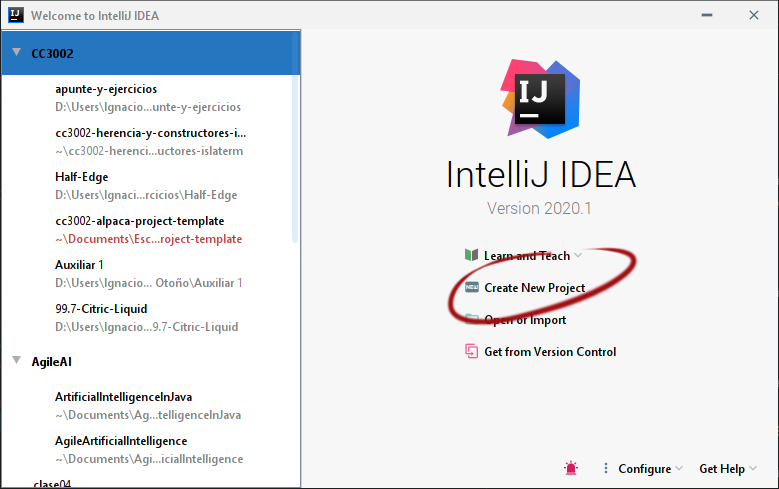
\includegraphics[width=0.7\textwidth]{img/Profundizando en Java/IntelliJ Landing.png}
    \caption{\textit{Landing view} de \textit{IntelliJ}}
    \label{fig:intellij-lv}
  \end{figure}

  Si ya abrieron algún proyecto con \textit{IntelliJ}, entonces lo más probable es que
  el \textit{IDE} vuelva a abrir el último proyecto en el que trabajaron.
  En ese caso, para crear un nuevo proyecto deben ir a \texttt{File | New... | Project} 
  (como en la figura \ref{fig:intellij-project-1}).

  \begin{figure}[ht!]
    \centering
    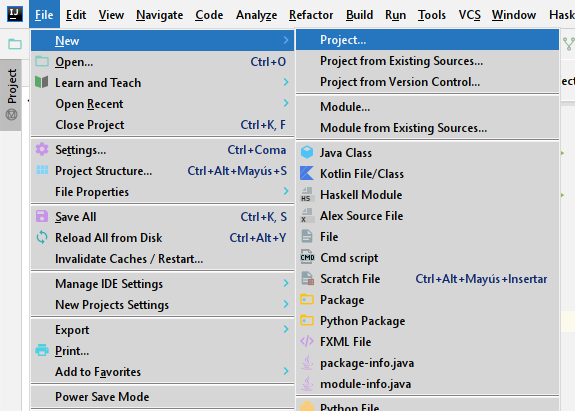
\includegraphics[
      width=0.7\textwidth
    ]{img/Profundizando en Java/IntelliJ Main Menu New Project.png}
    \caption{Crear un nuevo proyecto desde el menú principal de \textit{IntelliJ}}
    \label{fig:intellij-project-1}
  \end{figure}

  \newpage
  Una vez que hayan hecho lo anterior, entrarán al menú de creación de proyectos.
  Aquí se les presentaran muchas opciones (figura \ref{fig:intellij-project-2}), aquí 
  deben seleccionar el \textit{SDK} y las herramientas a utilizar en el proyecto, en el 
  ejemplo el \textit{SDK} es el 14 y no utilizaremos ninguna herramienta adicional.

  \begin{figure}[ht!]
    \centering
    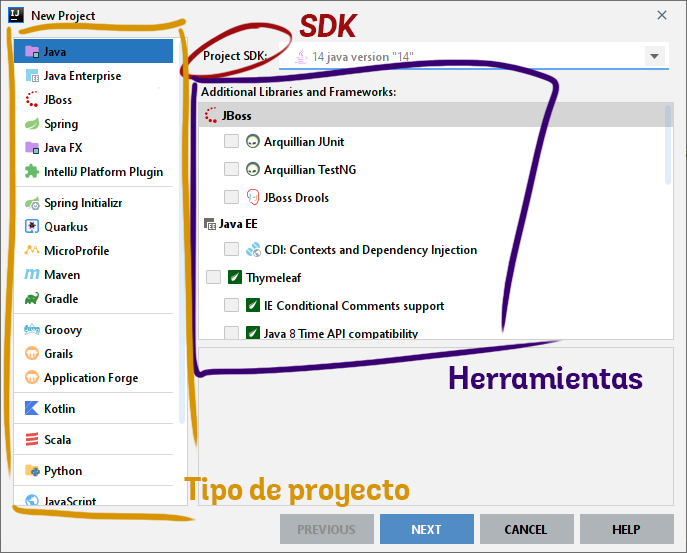
\includegraphics[
      width=0.7\textwidth
    ]{img/Profundizando en Java/IntelliJ Project Type.png}
    \caption{Menú de creación de proyecto: tipo de proyecto}
    \label{fig:intellij-project-2}
  \end{figure}

  Con estas opciones seleccionadas, den clic a \texttt{Next} para continuar al paso 
  siguiente de la creación del proyecto.

  La pestaña siguiente les dejará seleccionar un \textit{template} para comenzar un 
  proyecto con código predefinido.
  En este caso no utilizaremos ninguno, así que pueden saltarse esa vista.

  La última vista de la creación de proyecto es la que contiene los datos de nuestro proyecto, 
  aquí se puede elegir el nombre del proyecto y la ubicación donde se va a guardar, para este 
  capítulo crearemos un proyecto \textit{Bakemon} como se muestra en la figura 
  \ref{fig:intellij-project-3}.
  
  \begin{figure}[ht!]
    \centering
    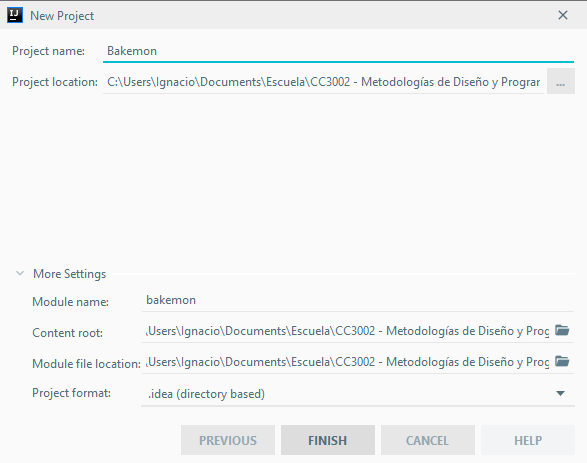
\includegraphics[
      width=0.7\textwidth
    ]{img/Profundizando en Java/IntelliJ Project Name.png}
    \caption{Menú de creación de proyecto: datos del proyecto}
    \label{fig:intellij-project-3}
  \end{figure}
%